

\chapter{Phenomenology of Processes}

\section[The process \ppwbblnbb]
{The process $\boldsymbol{\ppwbblnbb}$} \label{sec:wbbproduction}
%{The process $\boldsymbol{\mathbf{\ppwbblnbb}}$} \label{sec:wbbproduction}

%%%%%%%%%%%%%
\begin{figure}[!htb]
 \center
 \caption[Feynman diagrams for \ppwbblnbb]{
  The Feynman diagram for the process
   \ppwbblnbb is illustrated below,
   and is composed from the individual vertices 
   illustrated on the left, each of which is
   described in Section \ref{sec:wbbproduction}.
 } 
\begin{tabular}{rl}
 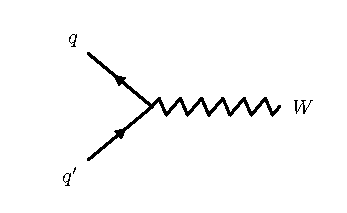
\includegraphics[width=0.3\textwidth]{/Users/rhombus/CMS/Thesis/thesis/pdfs/feyn/ppw/ppw.pdf} & 
 \multirow{3}{*}{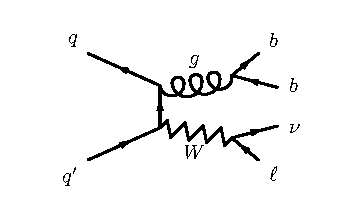
\includegraphics[width=0.6\textwidth]{/Users/rhombus/CMS/Thesis/thesis/pdfs/feyn/ppwbblnbb/ppwbblnbb.pdf}} \\
 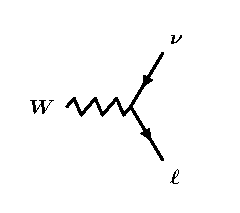
\includegraphics[width=0.3\textwidth]{/Users/rhombus/CMS/Thesis/thesis/pdfs/feyn/wln/wln.pdf} & {} \\
 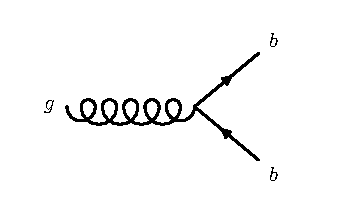
\includegraphics[width=0.3\textwidth]{/Users/rhombus/CMS/Thesis/thesis/pdfs/feyn/gbb/gbb.pdf} & {}
\end{tabular} 
    \label{fig:ppwbblnbbfeyn}
\end{figure}
%%%%%%%%%%%%%

 \subsection[\ppw]
 {$\boldsymbol{\ppw}$}

  The $W$ boson couples to all charged fermions
   and can be
   created during the collision of a quark-antiquark
   pair with a relative charge difference of $e$.
  In the proton are quarks and the most prevalant valence
   quark is the $u$.
  Therefore in a $pp$ collision,
   the channel by which most
   $W$ bosons are produced is
   via a the annihilation of a valence $u$ quark
   from one proton with 
   a $\overline{d}$ from the sea of the other,
   $u\overline{d}\rightarrow W^+$.
  Quarks of higher generation can also be found
   inside the sea as the result of gluons splitting into
   $q\overline{q}$ pairs, but all interactions
   are modified by a coefficient in the CKM matrix
   and higher generation mixing is thus suppressed.
  In this thesis, all modes of $pp\rightarrow W^\pm$ production are
   considered.

 \subsection[\wln]
 {$\boldsymbol{\wln}$}
  Just as the $W$ boson can be created by the
   collision $q\overline{q}'\rightarrow W$, 
   it can also decay as $W\rightarrow q\overline{q}'$.
  This is known as hadronic $W$ decay and
   can be a useful analysis channel for experimentalists,
   especially for decay products with energies approaching
   the \TeV scale.
  Leptonic $W$ decay, $\wln$, is also an important 
   channel for experimentalists and is the
   one considered in this analysis.
  Because leptons constitute a negligible fraction
   of the sea, the detection of leptons at high
   energy after a $pp$ collision is often a good 
   indicator of the decay of a massive gauge boson,
   $\wln$ or $Z\rightarrow \ell\overline{\ell}$.
  
  The $W$ boson is much heavier than any of the leptons
   and therefore decays with roughly equal probability
   to any of $e\nu_e, \mu\nu_\mu, \tau\nu_\tau$.
  From Table~\ref{tab:lifetimes}, tauons created
   at CMS
   subsequently decay before reaching the 
   detector, so for this analysis, the decay
   channel of the $W$ investigated is
   $\wln$ where $\ell\in e,\mu$.

 \subsection[\gbb]
 {$\boldsymbol{\gbb}$}
  Because quarks couple strongly to gluons
   and $q\overline{q}'\rightarrow W$ has been shown to be
   an important production channel in $pp$ collisions,
   it is possible for one of the
   initial state quarks to radiate a gluon.
  This is called initial state radiation, ISR,
   and if the gluon is produced with enough energy,
   it is capable of splitting to a quark-antiquark pair.
  In particular, a $g\rightarrow b\overline{b}$ vertex
   can be added to either of the incoming quarks.
  
%
% \subsection{b-jets}
%  quarks, jets/hadronization \\
%  heavy flavor - b quarks \\
%  displaced vertices
%

\section[The process \ppzgnng]
        {The process $\boldsymbol{\ppzgnng}$} \label{sec:znngproduction}

%%%%%%%%%%%%%
\begin{figure}[!htb]
 \center
 \caption[Feynman diagrams for \ppzgnng]{
  The Feynman diagram for the process
   \ppzgnng is illustrated below,
   and is composed from the diagrams 
   illustrated on the left, each of which is
   described in Section \ref{sec:znngproduction}.
 } 
\begin{tabular}{rl}
 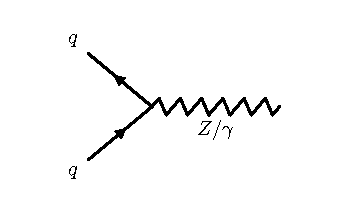
\includegraphics[width=0.3\textwidth]{/Users/rhombus/CMS/Thesis/thesis/pdfs/feyn/ppzsg/ppzsg.pdf} & 
 \multirow{3}{*}{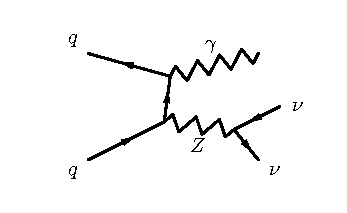
\includegraphics[width=0.6\textwidth]{/Users/rhombus/CMS/Thesis/thesis/pdfs/feyn/ppzgnng/ppzgnng.pdf}} \\
 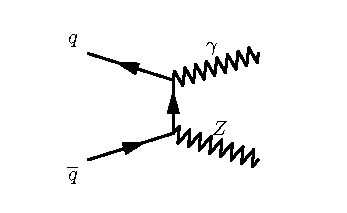
\includegraphics[width=0.3\textwidth]{/Users/rhombus/CMS/Thesis/thesis/pdfs/feyn/ppzg/ppzg.pdf} & {} \\
 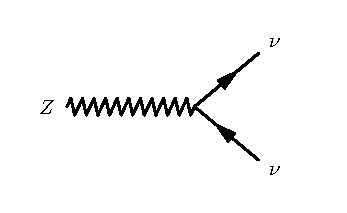
\includegraphics[width=0.3\textwidth]{/Users/rhombus/CMS/Thesis/thesis/pdfs/feyn/znn/znn.pdf} & {}
\end{tabular} 
    \label{fig:ppwbblnbbfeyn}
\end{figure}
%%%%%%%%%%%%%

 \subsection[\ppzsg]
 {$\boldsymbol{\ppzsg}$}

 Similar to the $W$ boson, the $Z$ boson and the photon can
  also each be produced via the collision of quarks in
  the process $q\overline{q} \rightarrow Z/\gamma$.
 Unlike interactions with the $W$ boson, 
  interactions with $Z/\gamma$ conserve parity invariance
  and do not transport charge.
 Any interaction which can happen as mediated
  by a photon can also happen with the exchange
  of a $Z$ boson, but for collisions at $\sqrt{s}<M_Z = 90$ \GeV,
  the $Z$ can not be made on-shell.
 In this low energy regime $\gamma$ exchange dominates,
  but in 2015, the LHC ran at $\sqrt{s}=13$ \TeV
  and the relative mass difference between the $Z$ and the $\gamma$
  played a negligible role in their relative rates of production. 

 \subsection[\ppzg]
 {$\boldsymbol{\ppzg}$}
 


 \subsection[\znn]
 {$\boldsymbol{\znn}$}





%%\chapter{$Wb\bar{b}$ Production}\label{sec:wbbproduction}
% The SM allows for the production of $W$ bosons
%  through the annihilation of a $u$-type quark
%  with a $d$-type quark which are already found
%  as valence quarks the proton.
% Because the charged current interactions do not
%  fully respect quark generations, 
%  the mixing of generations is possible,
%  but are suppressed via the %factors in the
%  Cabbibo-Kobayashi-Maskawa (CKM) matrix.
%  $u$ and $d$ quarks making up 

